% ==================================================================
%  Lessons 5 to 9: what a user sees, the clock, the ambiguities, and
%  the testing on simulated and real data.  Answers in answers_5_9.tex.
% ==================================================================

% ==================================================================
\section{What a user receives and sees}\label{sec:l5}
% ==================================================================

\paragraph{Goal.} Follow the corrections to a user: what it receives, what it
cannot see, and what may therefore be graded.

\paragraph{The idea.} A user positions itself with the equations of
\cref{sec:l1}, with the network's clock $C$, code bias $B$ and phase bias $P$ in
place of the satellite terms, and with its own receiver clock, slant ionosphere
and float ambiguities. The three null directions of \cref{sec:l1}, now at the
user's receiver, absorb three parts of the corrections: a change common to all
clocks of a system, a constant on a satellite's phase bias, and a geometry-free
offset of a satellite's code biases. These are the directions a reference choice
moves, so a user cannot see the choice (\cref{q:toy-user} showed it with numbers).
The S-system theory says the same of the correction covariance: its rank-one
clock and ionosphere parts ``lie in the user's own design range and are absorbed''
(\texttt{SBASIS-THEORY-E.md}, section E4). Hence standing invariant 5 of
\texttt{CLAUDE.md}: grade only datum-invariant or single-difference quantities.
The correction file declares its choices in a header line (the S line) and marks
every change of pivot with an epoch record (\texttt{E}, \texttt{datum\_changed=1}).

\begin{question}{absorb}{derive}{Three things a float user absorbs}{\ref{q:rx-clock} to \ref{q:rx-iono} and \ref{q:toy-user}}
Take the user's code and phase rows for satellite $\sat$ of system $g$, with
receiver clock, inter-system bias, slant ionosphere $I^\sat$ and float
ambiguities as unknowns, and the corrections applied.
\begin{enumerate}[leftmargin=*, itemsep=1pt]
\item Show that adding $\Delta$ to the clock $C$ of every satellite of system $g$
      changes no position.
\item Show that adding a constant $d$ to one satellite's phase bias changes no
      position, and say what changes instead.
\item Show that adding $(\delta, \mu_2\delta)$ to the two code biases of one
      satellite is absorbed, and say what that does to the user's ionosphere.
\item The status report's clock comparison (step 5) removes two means before it
      computes a standard deviation. Which two, and which of the three cases does
      each stand for?
\end{enumerate}
\end{question}

\begin{question}{sline}{read}{The header line of reference choices}{\ref{q:four}}
Line 2 of \texttt{runs/\_rf0hv15\_sim6/products.txt} is
\begin{cmd}
S,S30000SIM,1,nominal-wu93,0,0,1,0,0.05,1,COD0MGXFIN_20241290000_01D_05M_ORB.SP3+
  COD0MGXFIN_20241290000_01D_30S_CLK.CLK,E:E02,G:G01,cbjump=1,atx=igs20.atx,oref=CoM,
  discfrac=0.25,hsig=pc,cbpin=E:C1C-C5Q,cbpin=G:C1C-C2W,
  sat_gf_datum=broadcast_tgd,pbhold=2
\end{cmd}
(one line in the file). With the writer \texttt{src/core/products/NetworkProductIO.cpp}
(lines 465 to 602) and \texttt{include/products/NetworkProductEmitter.hpp}: what
does each field declare? Which fields are the reference choices of
\cref{sec:l4}? Which token does a current run add that this one lacks, and which
choice does the real-data run's S line leave undeclared?
\end{question}

\begin{question}{step}{measure}{A declared step, seen and absorbed}{\ref{q:toy-setchange} and \ref{q:absorb}}
Find the epochs at which the run declares a change of reference, then measure how
every GPS clock record moves across the GPS one (tow 276150):
\begin{cmd}
awk -F, '/^E,/ && $7=="1" {print NR": "$0}' runs/_rf0hv15_sim6/products.txt
C:/Python313/python.exe - <<'EOF'
import statistics as st
d, t = {}, None
for line in open('runs/_rf0hv15_sim6/products.txt'):
    f = line.rstrip('\n').split(',')
    if f[0] == 'E':
        t = round(float(f[2]) / 30) * 30
    elif f[0] == 'C' and f[1].startswith('G') and t in (276120, 276150):
        d.setdefault(f[1], {})[t] = float(f[2])
s = [v[276150] - v[276120] for v in d.values() if len(v) == 2]
print(len(s), 'satellites, mean step %.4f m, sd after the mean %.4f m'
      % (st.mean(s), st.pstdev(s)))
EOF
\end{cmd}
\begin{enumerate}[leftmargin=*, itemsep=1pt]
\item How large is the step of the GPS clock records, and how much of it is left
      after the per-system mean is removed?
\item Which move of \cref{q:toy-setchange} is this, and what absorbs it at a
      user?
\item Why would a grade of raw clock steps call this epoch a 1.6~m defect?
\end{enumerate}
\end{question}

\begin{question}{refsat}{measure}{The reference satellite in every chord}{\ref{q:toy-datums} and \ref{q:absorb}}
The network's double-difference trace (\texttt{network\_dd\_fractional.csv})
differences every satellite against one reference satellite.
\begin{enumerate}[leftmargin=*, itemsep=1pt]
\item Derive: if every satellite's error has variance $\sigma^2$ and the reference
      satellite's $\sigma_{\mathrm{ref}}^2$, what is the variance of one chord and
      the correlation between two chords?
\item Run (about 12~s) and compare the L1C error as traced and reference-free
      (median $|e|$ in cycles, and the share that rounds to the right integer),
      over all epochs and over the last quarter:
\begin{cmd}
C:/Python313/python.exe scripts/simnet_amb_integer.py runs/simnet60_quiet_col_24h \
    --run runs/_rf0hv15_sim6 --ref-free
\end{cmd}
\item Why does a grade on the traced chords report the reference satellite's
      error?
\end{enumerate}
\end{question}

\lessonbox{What this lesson establishes}{%
\begin{itemize}[leftmargin=*, itemsep=0pt, topsep=2pt]
\item A float user absorbs a system-common clock change, a constant on a phase
      bias and a geometry-free code-bias offset; the reference choice is
      invisible to it.
\item A declared step of 1.63~m on every GPS clock leaves 3~mm after the
      per-system mean: grade datum-invariant quantities, never raw steps.
\item A double difference built on one reference satellite carries that
      satellite's error in every chord: grade reference-free. For the meeting:
      every number in the report is graded this way.
\end{itemize}}

% ==================================================================
\section{The satellite clock in time}\label{sec:l6}
% ==================================================================

\paragraph{Goal.} See how the network ties each satellite clock to its past, what
the phase-clock hold passes to a user, and why the clock's precision today is the
a priori clock product's.

\paragraph{The idea.} Three mechanisms shape the per-satellite part of the
clock, the part a user cannot absorb.
\begin{enumerate}[leftmargin=*, itemsep=1pt]
\item \emph{The temporal anchor} (card Q3, \texttt{network.clock\_temporal\_anchor}).
      Without it the clock is re-estimated from each epoch's data: the step
      between epochs was 9.23~cm per 30~s, because the clock's own process noise
      (\texttt{sat\_clock\_q}, $10^{-3}$~m$^2$/s) never binds. The anchor folds the
      previous epoch's clock in as a prior with variance
      $\max(\mathrm{var} + q\,\Delta t,\ \mathrm{floor})$ and
      \texttt{clock\_anchor\_q} $= 2.9\times10^{-8}$~m$^2$/s, a value measured from
      the clock's structure function (\cref{fig:l6-clock}, left).
\item \emph{The exact coupling update} (card CTU,
      \texttt{carry\_coupling\_exact\_update}). Carried station rows used to age the
      clock at $10^{-3}$~m$^2$/s while the shared solve folded it at
      $2.9\times10^{-8}$; the level froze. The exact update lets it converge at the
      anchor's rate (\cref{fig:l6-clock}, right).
\item \emph{The phase-clock hold} (cards PBH and LAH,
      \texttt{emit\_pb\_hold\_phase\_clock}). Between declared resets the network
      keeps each satellite's clock minus phase bias, $C - P$, constant up to a
      common mode, so a user's phase rows follow the a priori clock.
\end{enumerate}
Card SCB (24~October) made the consequence measurable on a simulated data set with
injected satellite clock error (offset $\sigma$ 0.5~m, rate $\sigma$
$10^{-5}$~m/s, random walk $3\times10^{-8}$~m$^2$/s).

\begin{figure}[h]
\centering
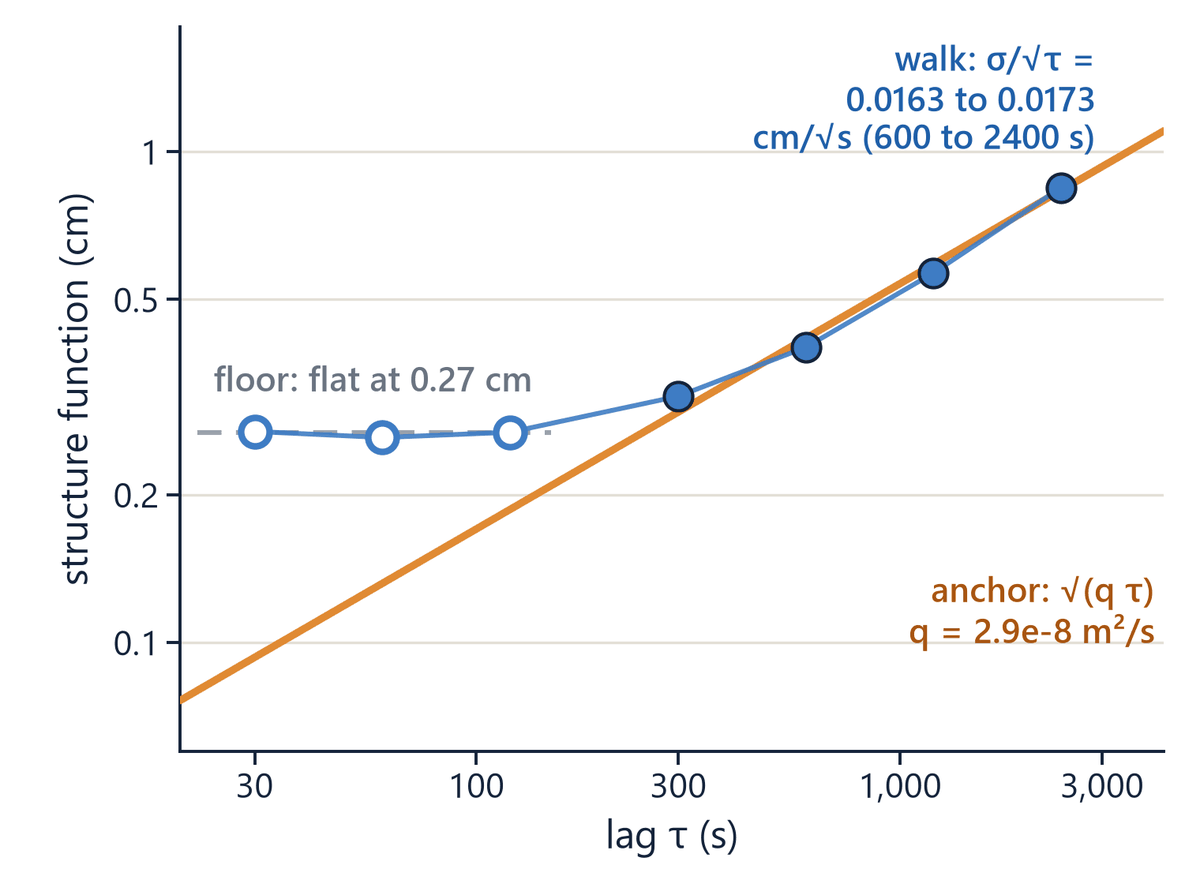
\includegraphics[width=0.44\linewidth]{clock_structure_function.png}\hfill
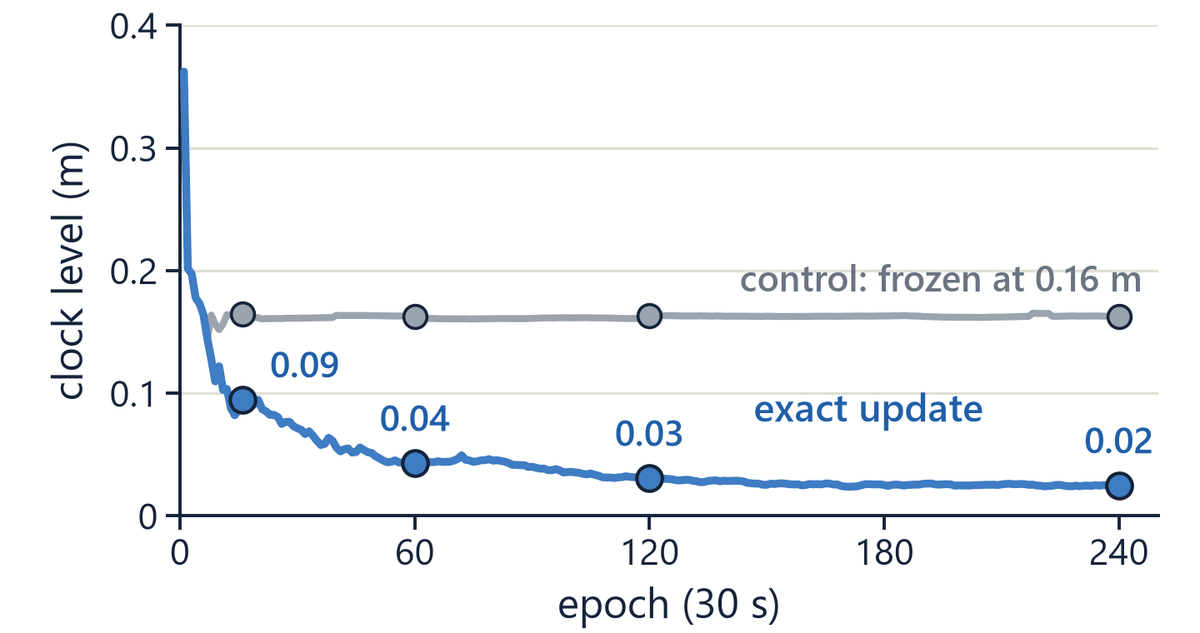
\includegraphics[width=0.54\linewidth]{sim_clock_level_update.png}
\caption{Left: structure function of the network's satellite clock correction
against lag: a floor of 0.27~cm from 30 to 120~s, then growth along the anchor's
line $\sqrt{q\tau}$, $q = 2.9\times10^{-8}$~m$^2$/s (deck slide 11). Right:
simulated network, error of the clock level by epoch, graded from 00:30:15: the
control freezes at 0.16~m, the exact coupling update falls to 0.02~m by epoch 240
(deck slide 10).}
\label{fig:l6-clock}
\end{figure}

\begin{question}{qstep}{derive}{A spectral density as a step}{}
\texttt{clock\_anchor\_q} is $2.9\times10^{-8}$~m$^2$/s and the epoch 30~s.
\begin{enumerate}[leftmargin=*, itemsep=1pt]
\item What is the $1\sigma$ random-walk step per epoch, and the $1\sigma$
      accumulation over 6~h?
\item The injected rate on the clock data set has $\sigma$ $10^{-5}$~m/s, 0.30~mm
      per epoch, which card SCB calls ``inside the golden anchor's permitted
      0.93~mm per epoch''. After how many epochs does a $10^{-5}$~m/s drift exceed
      the walk's $1\sigma$ accumulation? Why does comparing step sizes not
      guarantee that the anchor follows the drift?
\end{enumerate}
\end{question}

\begin{question}{tau}{derive}{A spectral density as a time constant}{\ref{q:qstep}}
Treat the anchored clock as a scalar random walk observed once per epoch with
noise variance $R = (9.23~\mathrm{cm})^2/2$ (the pre-anchor step is the difference
of two independent epoch estimates). Use the steady-state gain
$K = \sqrt{q\,\Delta t/R}$ of \texttt{docs/cards/raim-qc/DAY129-FRAME-ANATOMY.md}
(lines 138 to 143).
\begin{enumerate}[leftmargin=*, itemsep=1pt]
\item What are $K$ and the time constant $\Delta t/K$?
\item What error does a $10^{-5}$~m/s drift leave? Compare with the coefficient
      card SCB measured for the reference configuration, 2127~s.
\item What does the same argument give for the self-contained regime's
      $q = 5\times10^{-6}$~m$^2$/s? Card SCB measured 52~s.
\end{enumerate}
\end{question}

\begin{question}{hold}{derive}{What the phase-clock hold passes to the user}{\ref{q:absorb} and \ref{q:qstep}}
\texttt{include/network/emit/PbHold.hpp} (lines 60 to 66) writes the held phase
bias of a satellite as $P(t) = p(t_0) + [\tilde c(t) - \tilde c(t_0)]$, with
$\tilde c = c - M$ the estimated clock minus its system mean.
\begin{enumerate}[leftmargin=*, itemsep=1pt]
\item Show what $C - P$ is between resets, and what a user's phase rows see when
      the a priori clock is $a(t)$ and the truth $a(t) + e(t)$.
\item On the clock data set $e(t)$ is a rate ($\sigma$ $10^{-5}$~m/s) plus a random
      walk ($3\times10^{-8}$~m$^2$/s). What rms error does the hold pass to the
      phase rows in hour 6 (5 to 6~h after the reset)? Card SCB, section 8,
      measured 0.201~m for GPS.
\item Lines 311 to 319 of \texttt{src/core/config/GnssConfigLoadNetwork.cpp}
      enforce a precondition on the hold. Which, and why does part 1 make it
      necessary? Which token of the S line declares the hold in force?
\end{enumerate}
\end{question}

\begin{question}{postures}{measure}{Two postures on the clock data set}{\ref{q:tau} and \ref{q:hold}}
Run the clock grader on the reference case and on the self-contained regime, both
on the clock data set (a few seconds each):
\begin{cmd}
C:/Python313/python.exe -B scripts/simnet_clock_truth_grade.py \
    --fixture D:/GnssProcessorSupport/fixtures/simnet60_clk_col_24h \
    --run D:/GnssProcessorSupport/runs_nom/_rap_scb_g_k6
C:/Python313/python.exe -B scripts/simnet_clock_truth_grade.py \
    --fixture D:/GnssProcessorSupport/fixtures/simnet60_clk_col_24h \
    --run D:/GnssProcessorSupport/runs_nom/_rap_scb_c_k6
\end{cmd}
Read for each the clock level at hour 6, the rms of the per-satellite mean
errors, the correlation of the mean error with the drawn rate, and the user's
hourly error in hours 3 to 6. Which posture follows the drift? Why is the
reference case's user error so much larger than its clock error? What do these
lines not show?
\end{question}

\begin{question}{nbp}{derive}{The cost of leaving the final clock, on real data}{\ref{q:postures}}
Card NBP, section 12 (lines 212 to 219), splits the cost of the native
broadcast-clock posture over days 130 to 132 into three steps: the self-contained
regime $+0.0024$~m, removing satellite G01 $-0.0007$~m, the broadcast clock in place
of CODE's $+0.0099$~m. The pooled median of the whole change is $+0.0171$~m (line
176).
\begin{enumerate}[leftmargin=*, itemsep=1pt]
\item Why do the steps not add to the total? Which part is the clock's
      information?
\item Against which reference configuration, which days and which hours was the
      1.7~cm measured, and what does the first hour add?
\end{enumerate}
\end{question}

\lessonbox{What this lesson establishes}{%
\begin{itemize}[leftmargin=*, itemsep=0pt, topsep=2pt]
\item $q = 2.9\times10^{-8}$~m$^2$/s is a 0.93~mm step per epoch and, against the
      epoch noise, a time constant of about 35~min.
\item The phase-clock hold hands a user the a priori clock's motion: a wrong a
      priori clock reaches the phase rows one to one, so the hold is valid only
      with a precise a priori clock.
\item The self-contained postures estimate the clock to about 2~cm on simulated
      error but are not armed; on real data, replacing CODE's clock costs 1.7~cm
      at the median. For the meeting: the clock's precision is CODE's.
\end{itemize}}

% ==================================================================
\section{Float ambiguities and integers}\label{sec:l7}
% ==================================================================

\paragraph{Goal.} See why the network keeps its ambiguities float, what a complete
set of integers would buy, and why the corrections carry no integers yet.

\paragraph{The idea.} In the uncombined model every phase row carries both the
slant ionosphere and an ambiguity, and on GPS L1 and L2 the two enter in nearly
the same direction: a common L1 and L2 cycle moves the phase by $(\lambda_1,
\lambda_2) = (0.1903, 0.2442)$~m, the ionosphere along $(1, \mu_2)$ with $\mu_2 =
1.6469$. With a free slant ionosphere per line of sight, the integers become
visible only once the double-differenced ionosphere is known to about 0.1 L1
cycle. The re-founding chose the \emph{float vehicle} (card RF-1): each ambiguity
is a float state of its station block with a joint covariance, a floored birth
prior and zero process noise; integers are graded, not fixed. \Cref{q:toy-user}
showed where a user's integer property comes from: the network's pins.

\begin{figure}[h]
\centering
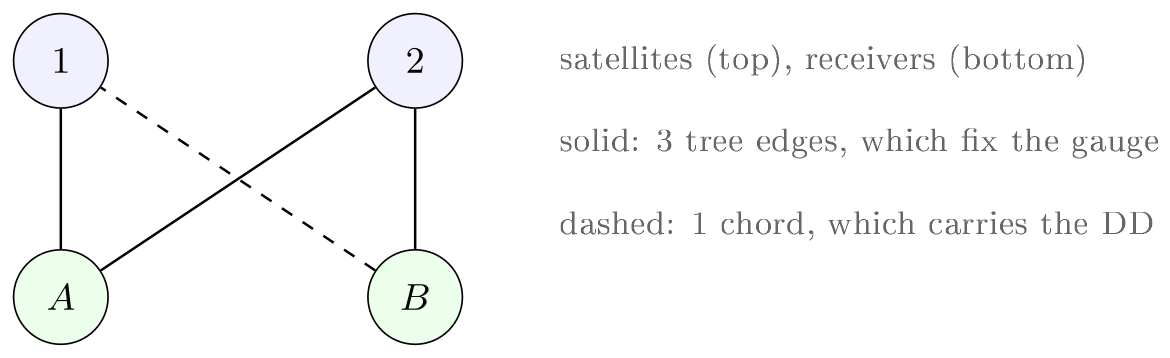
\includegraphics[width=0.46\linewidth]{observation_graph_cycle.png}\hfill
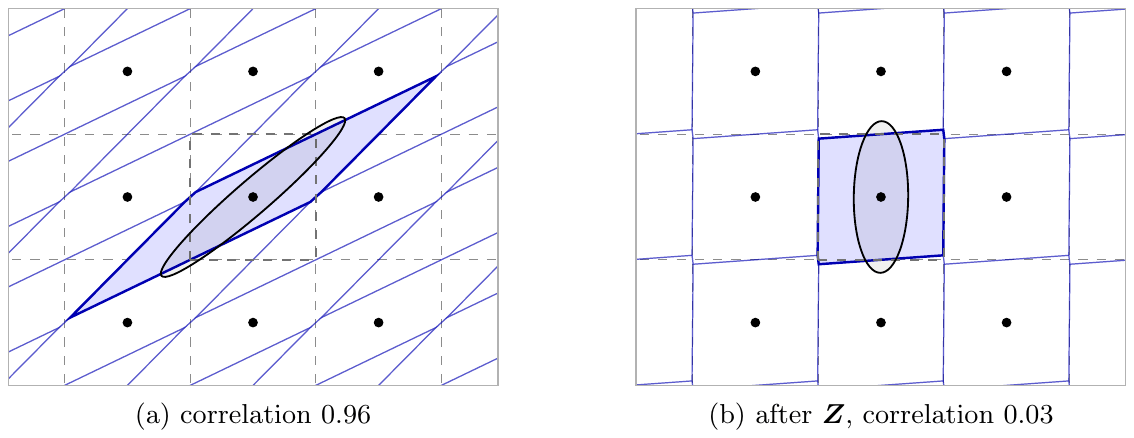
\includegraphics[width=0.5\linewidth]{pull_in_regions.png}
\caption{Left: the smallest observation graph with a cycle: satellites 1 and 2
(top), receivers $A$ and $B$ (bottom); the three solid arcs form a spanning tree
whose ambiguities the reference choice fixes, the dashed chord carries the one
double difference the data determine (\texttt{docs/report/network\_carry.tex},
figure 1). Right: a two-dimensional integer search; at correlation 0.96 the error
ellipse is long and the search's pull-in region a long parallelogram, unlike the
rounding squares (dashed); after the decorrelating transformation $\bm{Z}$ the
two nearly agree (\texttt{docs/report/linear\_algebra.tex}, figure 3; a generic
example).}
\label{fig:l7}
\end{figure}

\begin{question}{nl}{derive}{Why an integer is mostly ionosphere}{\ref{q:rx-phase} and \ref{q:rx-iono}}
From $f_1 = 1575.42$~MHz and $f_2 = 1227.60$~MHz, compute $\lambda_1$, $\lambda_2$
and $\mu_2$, the angle between the ionosphere direction $(1, \mu_2)$ and the
common-cycle direction $(\lambda_1, \lambda_2)$ in metres of phase, its cosine,
and the part of one common L1 and L2 cycle that is orthogonal to the ionosphere.
Card ARL (line 43) calls a narrow-lane integer ``99.3\,\% ionosphere''. Is that a
share of amplitude or of variance?
\end{question}

\begin{question}{cycles}{derive}{An ionosphere error in cycles}{\ref{q:nl}}
A double-difference L1 ionosphere error $d$ (metres) is absorbed by the
ambiguities.
\begin{enumerate}[leftmargin=*, itemsep=1pt]
\item What are the L1 and wide-lane ($L1 - L2$) errors in cycles for
      $d = 0.4233$~m (no pin) and $d = 0.0419$~m (every ambiguity pinned)? Check
      the factors against \texttt{docs/cards/raim-qc/T3-IONO-MECHANISM.md} (lines
      326 to 331).
\item Instantaneous resolution needs about 0.1 L1 cycle. What is that in metres
      and in TECU, and by what factor does the no-pin case miss it?
\end{enumerate}
\end{question}

\begin{question}{pins}{derive}{Integer pins and float pins}{\ref{q:toy-user} and \ref{q:four}}
Work \cref{q:toy-user} in cycles, with a receiver phase bias $\beta_\rx$ (the same
for every satellite), so that $N^\sat_\rx = z^\sat_\rx + \beta_\rx$ with
$z^\sat_\rx$ an integer. Let the network pin $N^\sat_A \equiv \zeta^\sat$ instead of 0.
\begin{enumerate}[leftmargin=*, itemsep=1pt]
\item What does the network emit as $\bar b^\sat$, and what does the user $C$
      estimate as $\tilde N^\sat_C$?
\item Form the difference between satellites $\sat$ and $k$ at $C$. When is it an
      integer?
\item The reference configuration pins each anchor ambiguity at its own float
      value (\texttt{docs/network\_ambiguity\_resolution\_design.md}, line 335).
      What does part 2 predict for its corrections? What does card IRD (sections
      1 to 3) propose instead?
\end{enumerate}
\end{question}

\begin{question}{oracle}{read}{Complete and partial pins}{\ref{q:cycles}}
Read sections 0 and 8.1 of \texttt{docs/SPEC\_oracle\_pin.md}. What is the
``integer-information deficit'', which row of its table carries it, and why is the
raw per-line-of-sight error (2.73~m) the wrong row? What do the partial pins
(L5Q alone; L1C with L2W; one station; one satellite) show, and on which simulated
data set were the numbers produced?
\end{question}

\begin{question}{null}{measure}{Integers in the float, none in the corrections}{\ref{q:pins}}
Run (each under 10~s):
\begin{cmd}
C:/Python313/python.exe scripts/simnet_wire_integer_consistency.py \
    runs/simnet60_quiet_col_24h --run runs/_rf0hv15_sim6 --bands L1C,L2W \
    --systems G --wl --nl --null-mc 500 --start-hms 00:30:15
C:/Python313/python.exe scripts/simnet_producer_ar_grade.py runs/simarl_r2 \
    --run runs/_rap_arl_r2dp --settle-h 1
\end{cmd}
The first grades the published GPS phase biases for integer consistency (the
fraction of wide-lane and narrow-lane combinations against a uniform null; a set
of perfect corrections reads 0.000). The second grades the log-only integer search
of card ARL. What does each print, and what do the two together say about where
the integers are?
\end{question}

\lessonbox{What this lesson establishes}{%
\begin{itemize}[leftmargin=*, itemsep=0pt, topsep=2pt]
\item An L1 and L2 integer step lies $6.66^\circ$ from the ionosphere direction;
      with a free slant ionosphere the integers need a double-differenced
      ionosphere to 0.117~TECU.
\item A user's between-satellite ambiguity is an integer only if the network's
      pins are integers; the reference configuration pins float values, so its
      corrections sit at the uniform null.
\item The network's float solution holds integers (a log-only search fixes 42\,\%
      on a simplified simulation, none wrongly). For the meeting: no integers are
      published or fixed on real data.
\end{itemize}}

% ==================================================================
\section{Testing on simulated data}\label{sec:l8}
% ==================================================================

\paragraph{Goal.} See what the simulated network certifies, where a simulated run
starts and is graded, and how much error the network adds above the user's own
floor.

\paragraph{The idea.} The simulated data set \texttt{runs/simnet60\_quiet\_col\_24h}
holds 60 network stations and the test station SZZ000SIM at 30~s from 00:00:30
(\cref{fig:l8}, left). It is \emph{quiet}: no cycle slips and no satellite clock
error, because its truth clock is the CODE product that the network also takes as
its a priori clock. The simulator extrapolated the satellite positions outside its
SP3 window for its first epochs; the reference case is graded from 00:30:15. The
network reports clocks and biases in its own reference choices, so truth is moved
into that basis before any comparison. The simulator also writes a set of perfect
corrections, so the same test station can be positioned with both sets
(\cref{fig:l8}, right).

\begin{figure}[h]
\centering
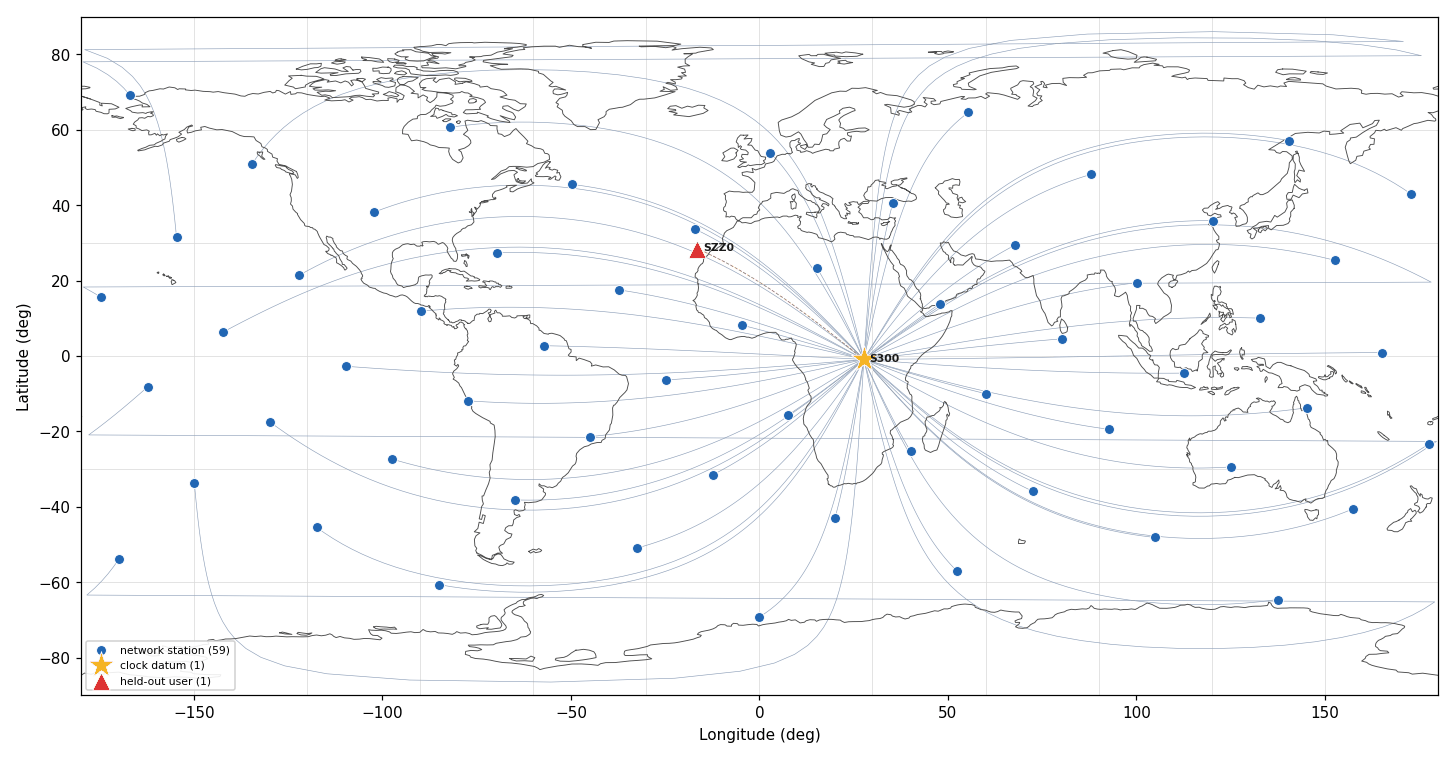
\includegraphics[width=0.42\linewidth]{sim_network_map.png}\hfill
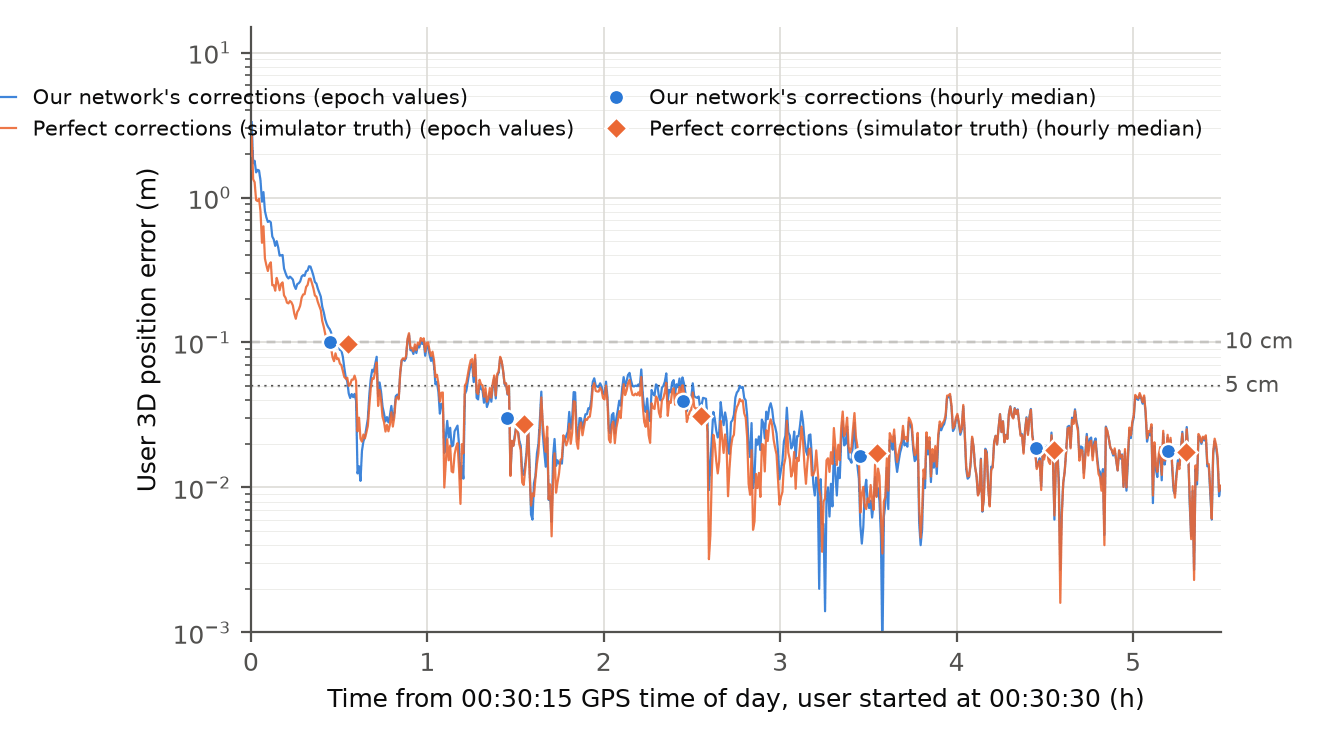
\includegraphics[width=0.56\linewidth]{sim_user_restarted.png}
\caption{Left: the simulated network, 59 stations and the clock-datum station
S30000SIM (star); the test station SZZ000SIM (triangle) is left out (deck slide
15). Right: SZZ000SIM with our network's corrections (blue) and with perfect
corrections (orange), user started at 00:30:30; lines are epochs, markers hourly
medians (\texttt{results/t2/plain/t2\_sim\_floor\_restart.png}).}
\label{fig:l8}
\end{figure}

\begin{question}{quiet}{read}{What the quiet simulation cannot test}{\ref{q:hold}}
Read card SCB, section 1 and the start of section 2 (lines 17 to 25), and
\texttt{results/t2/results.md} (lines 123 to 126). What makes the clock untestable
on the quiet data set, and what does its 0.9~cm agreement certify instead? Check
the absence of injected clock error directly:
\begin{cmd}
ls runs/simnet60_quiet_col_24h/*/truth_satclock.csv 2>/dev/null | wc -l
ls D:/GnssProcessorSupport/fixtures/simnet60_clk_col_24h/*/truth_satclock.csv | wc -l
\end{cmd}
\end{question}

\begin{question}{start}{derive}{Where a simulated run starts}{}
\begin{enumerate}[leftmargin=*, itemsep=1pt]
\item The data set's first epoch is tow 259230 (00:00:30). An epoch is reached when
      its elapsed time since the first epoch is at least the offset
      (\texttt{include/math/TimeUtils.hpp}, lines 416 to 448). At which tow and
      time do \texttt{network.start\_offset\_hours} 0.504167 and 0.4958333333 start
      a run? What does the ``half-epoch back-off'' do?
\item Count the extrapolated epochs. The geometry log warns only when the
      extrapolation exceeds half the SP3 interval
      (\texttt{src/core/model/ModelGeometry.cpp}, line 1204):
\begin{cmd}
grep "Position extrapolation" \
    runs/simnet60_quiet_col_24h/SZZ000SIM/logs/geometry.log \
  | sed -E 's/.*tow ([0-9.]+):.*/\1/' \
  | awk '{c[int(($1+15)/30)*30]++} END{for(e in c) print e,c[e]}' | sort -n
\end{cmd}
      How many epochs are logged, how many precede the SP3 window (which opens at
      tow 259500), and is ``faulty in the first 30 minutes'' the right description?
\end{enumerate}
\end{question}

\begin{question}{basis}{measure}{The published baseline's clock in the network's basis}{\ref{q:cbdatum}, \ref{q:absorb} and \ref{q:start}}
Run the clock grader on the published simulated baseline (started 00:00:30) and on
card SCB's quiet case (started 00:31:00):
\begin{cmd}
C:/Python313/python.exe -B scripts/simnet_clock_truth_grade.py \
    --fixture runs/simnet60_quiet_col_24h --run runs/_rf0hv15_sim6 --hours 6
C:/Python313/python.exe -B scripts/simnet_clock_truth_grade.py \
    --fixture runs/simnet60_quiet_col_24h \
    --run D:/GnssProcessorSupport/runs_nom/_rap_scb_g_q6
\end{cmd}
Compare the clock level by hour and the rms of the per-satellite mean errors.
Rerun the first with \texttt{--no-ds}: what does the datum share remove, and why
is it added to the truth rather than subtracted from the estimate? Why does the
first run's user not show its per-satellite constants?
\end{question}

\begin{question}{floor}{derive}{The network's cost and the user's floor}{\ref{q:start}}
From \texttt{results/t2/results.md} (lines 195 to 206), the hourly 3D medians with
the user restarted at 00:30:30, in metres: perfect corrections 0.0983, 0.0275,
0.0311, 0.0173, 0.0181, 0.0176; our network 0.1013, 0.0301, 0.0396, 0.0166, 0.0186,
0.0178. Compute the network's cost per hour, the largest cost and the floor in
hours 4 to 6. In which component does the floor sit (\texttt{results/t2/metrics.csv})?
\end{question}

\lessonbox{What this lesson establishes}{%
\begin{itemize}[leftmargin=*, itemsep=0pt, topsep=2pt]
\item The quiet simulation has no clock error to estimate; it certifies the
      algebra and the biases.
\item Nine epochs are extrapolated; 00:30:15 is a grading origin, and a run
      started at 00:00:30 keeps per-satellite clock constants of 0.32~m that no
      float user can see.
\item With perfect corrections as the control, the network adds at most 0.9~cm;
      the 1.7 to 1.8~cm floor is the user side's, in the height. For the
      meeting: one realization, no slips, no clock error.
\end{itemize}}

% ==================================================================
\section{Real data, and what may be claimed}\label{sec:l9}
% ==================================================================

\paragraph{Goal.} Grade the real-data result the way the project does, and put the
course together into what the presentation may claim.

\paragraph{The idea.} The real-data reference case
(\texttt{config/golden/golden\_field\_refound.json}, run \texttt{runs/\_rf0hv15\_field6})
processes 58 IGS stations on 8 May 2024, GPS L1/L2 and Galileo E1/E5a. The test
station WTZZ00DEU is left out of the network and positioned as a moving receiver
from the clock and bias records, without integer fixing and with its own float
ionosphere; it shares its site with two network stations. Sixteen further
stations, none of them in the network, are positioned from the same file
afterwards. A change is graded against the baseline pair and an unchanged copy run
by the same software, on the test station by hour and on the 16 stations, never on
one alone; the first hour is excluded from settled claims (\texttt{CLAUDE.md},
``Network runs: start from a golden'').

\begin{figure}[h]
\centering
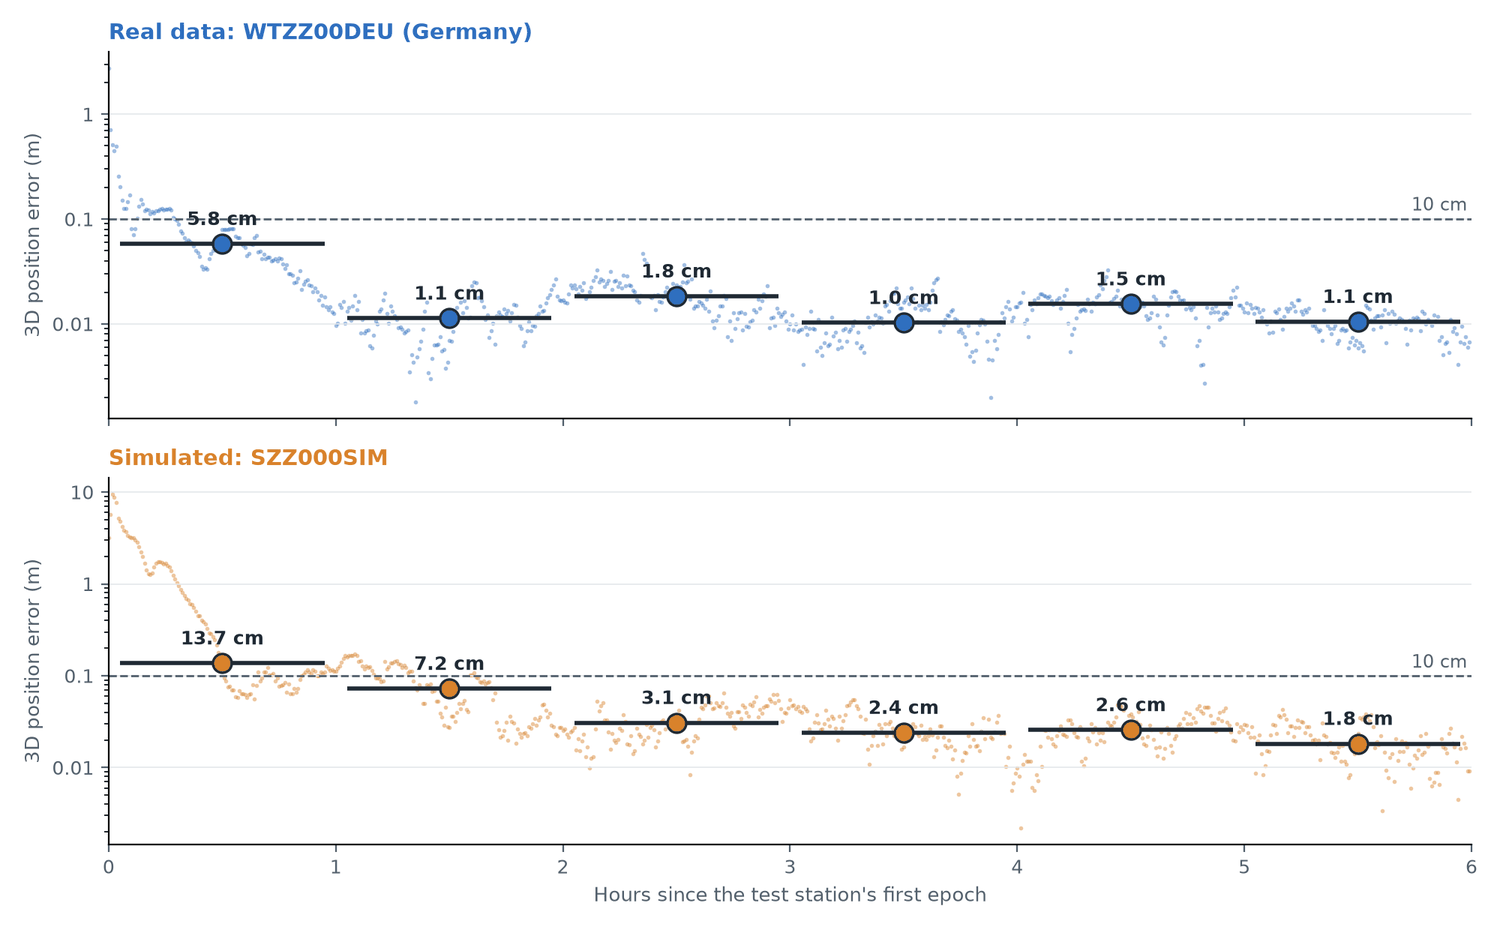
\includegraphics[width=0.5\linewidth]{test_station_by_hour.png}\hfill
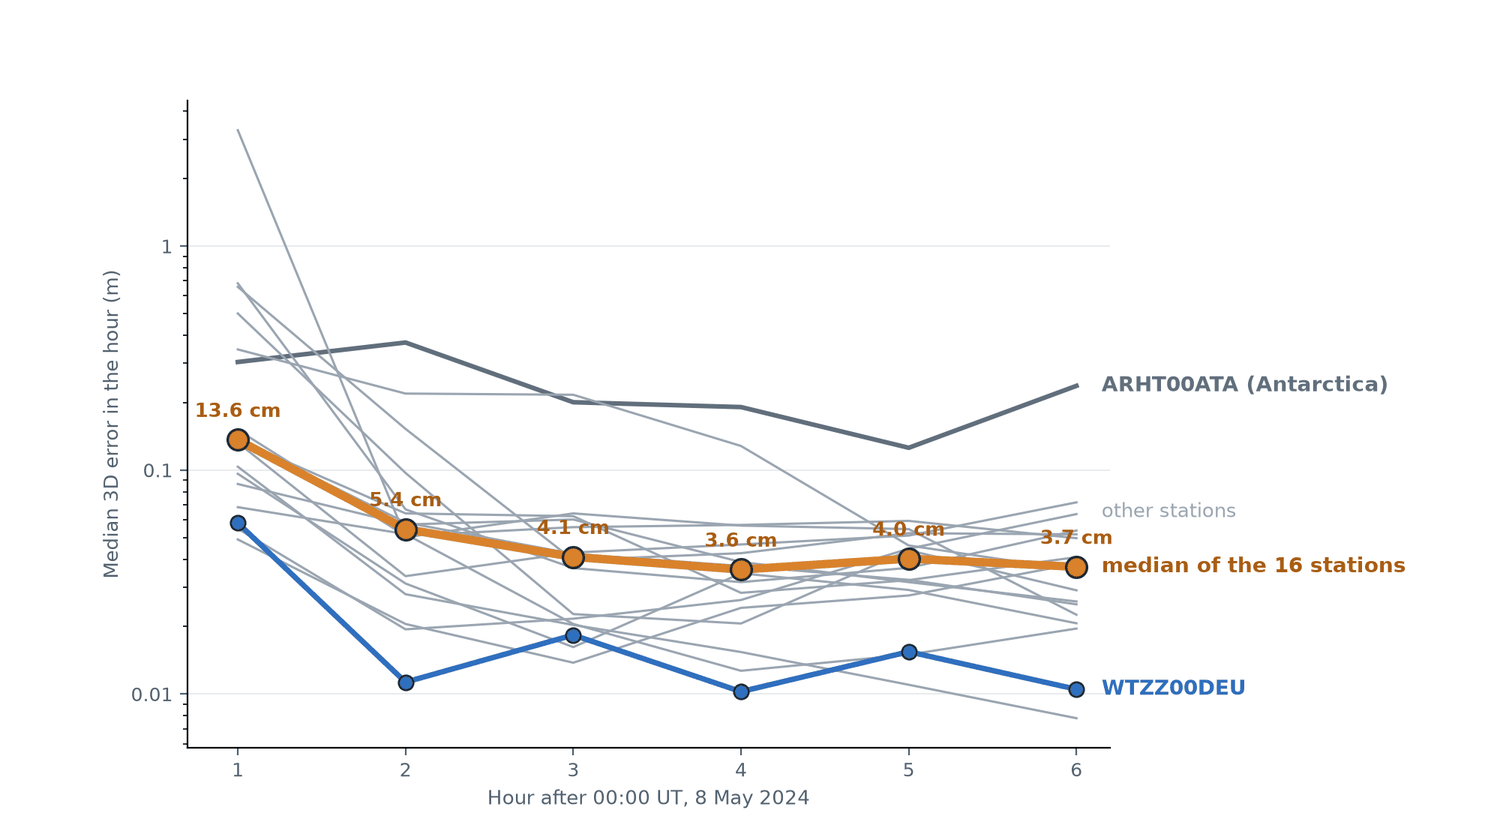
\includegraphics[width=0.48\linewidth]{sixteen_stations.png}
\caption{Left: the test station with our network's corrections, real data
(WTZZ00DEU, top) and simulated (SZZ000SIM, bottom); dots are epochs, bars hourly
medians. Right: hourly median for the 16 further stations (grey), their median
(orange), WTZZ00DEU (blue) and ARHT00ATA (dark). Status report figures.}
\label{fig:l9-a}
\end{figure}

\begin{figure}[h]
\centering
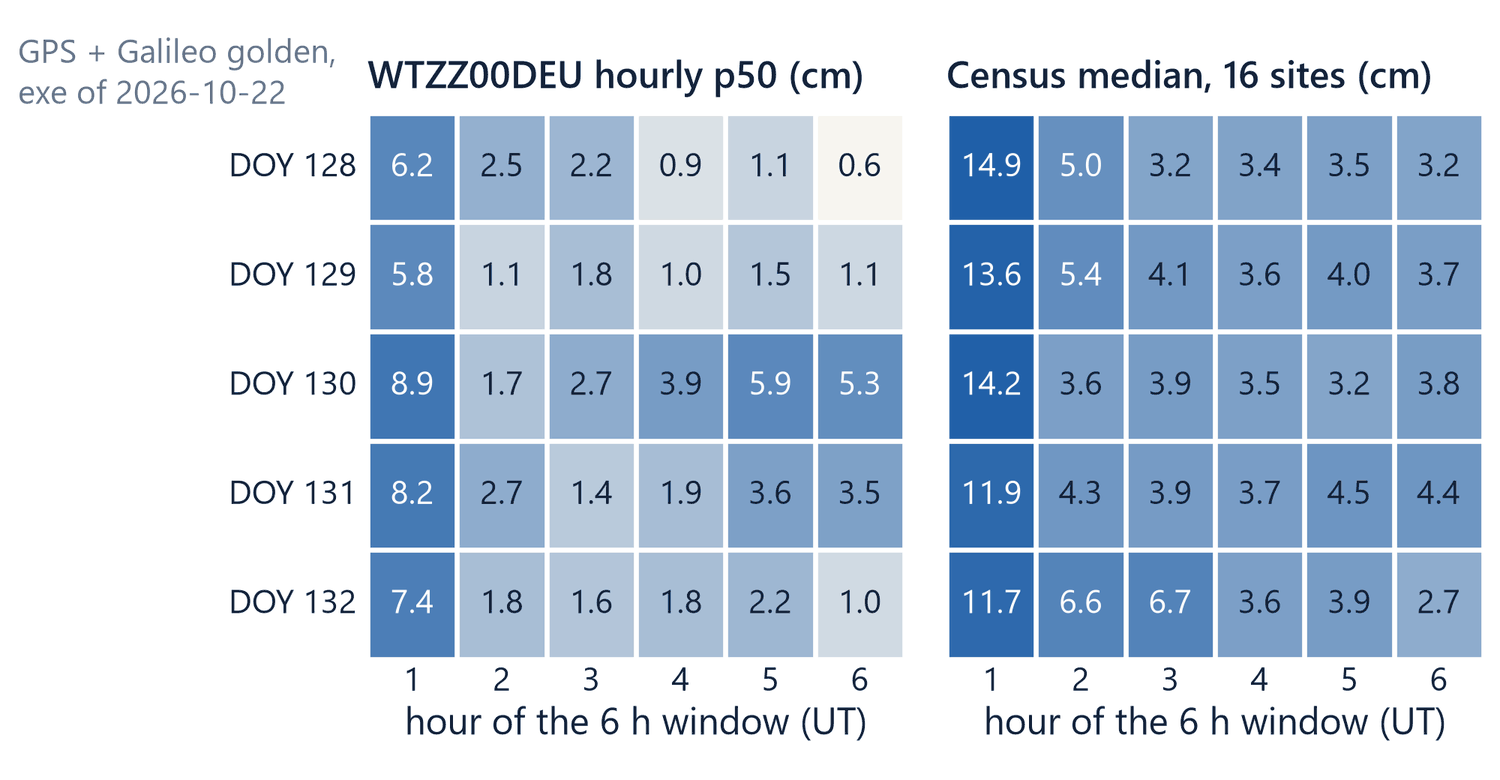
\includegraphics[width=0.52\linewidth]{five_days.png}\hfill
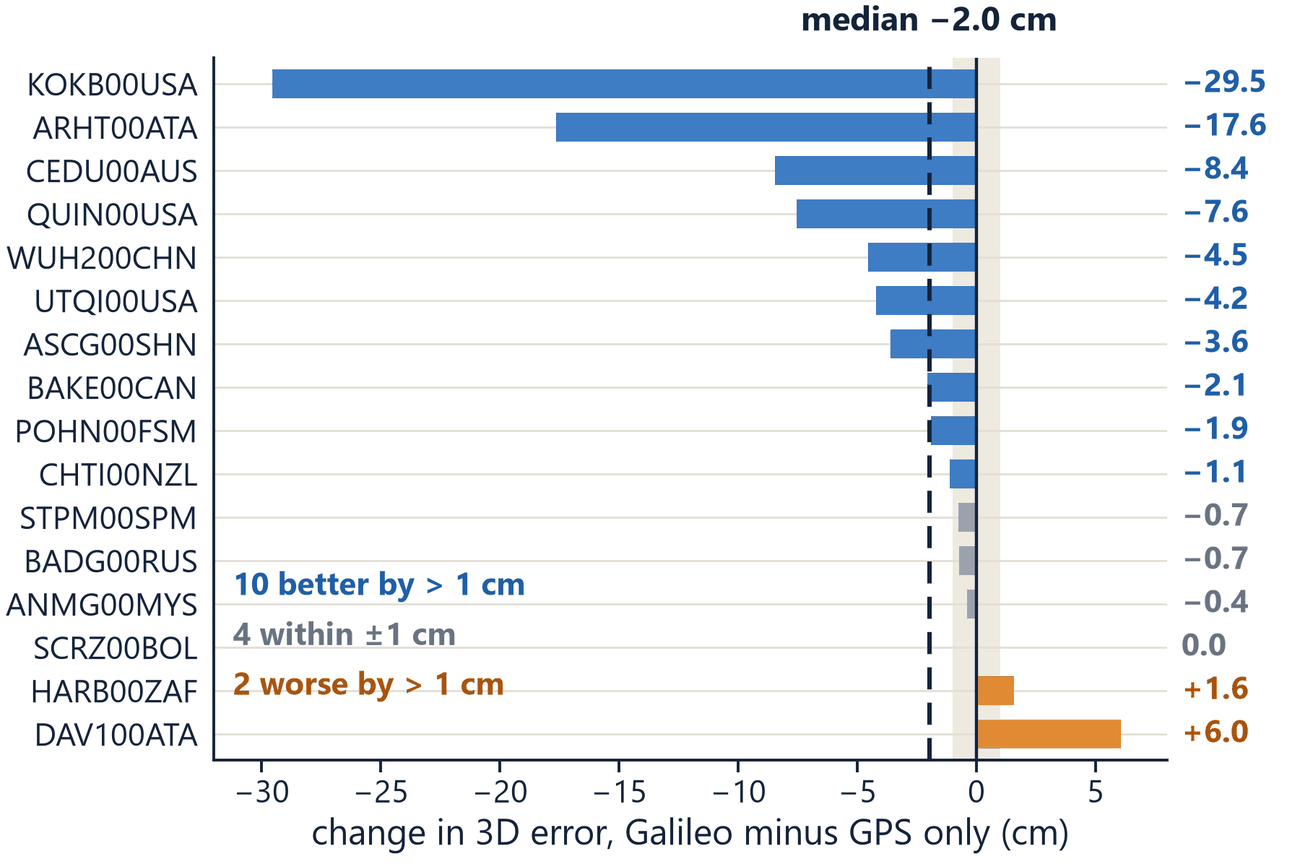
\includegraphics[width=0.46\linewidth]{galileo_change_per_station.png}
\caption{Left: five days, 7 to 11 May 2024, hourly median in cm: WTZZ00DEU and the
median of the 16 stations (the labels ``golden'' and ``census'' are the record's
names for the reference configuration and the 16 stations; deck slide 33). Right:
change of each station's error in hours 2 to 6 when Galileo is added, median
$-2.0$~cm (deck slide 19).}
\label{fig:l9-b}
\end{figure}

\begin{figure}[h]
\centering
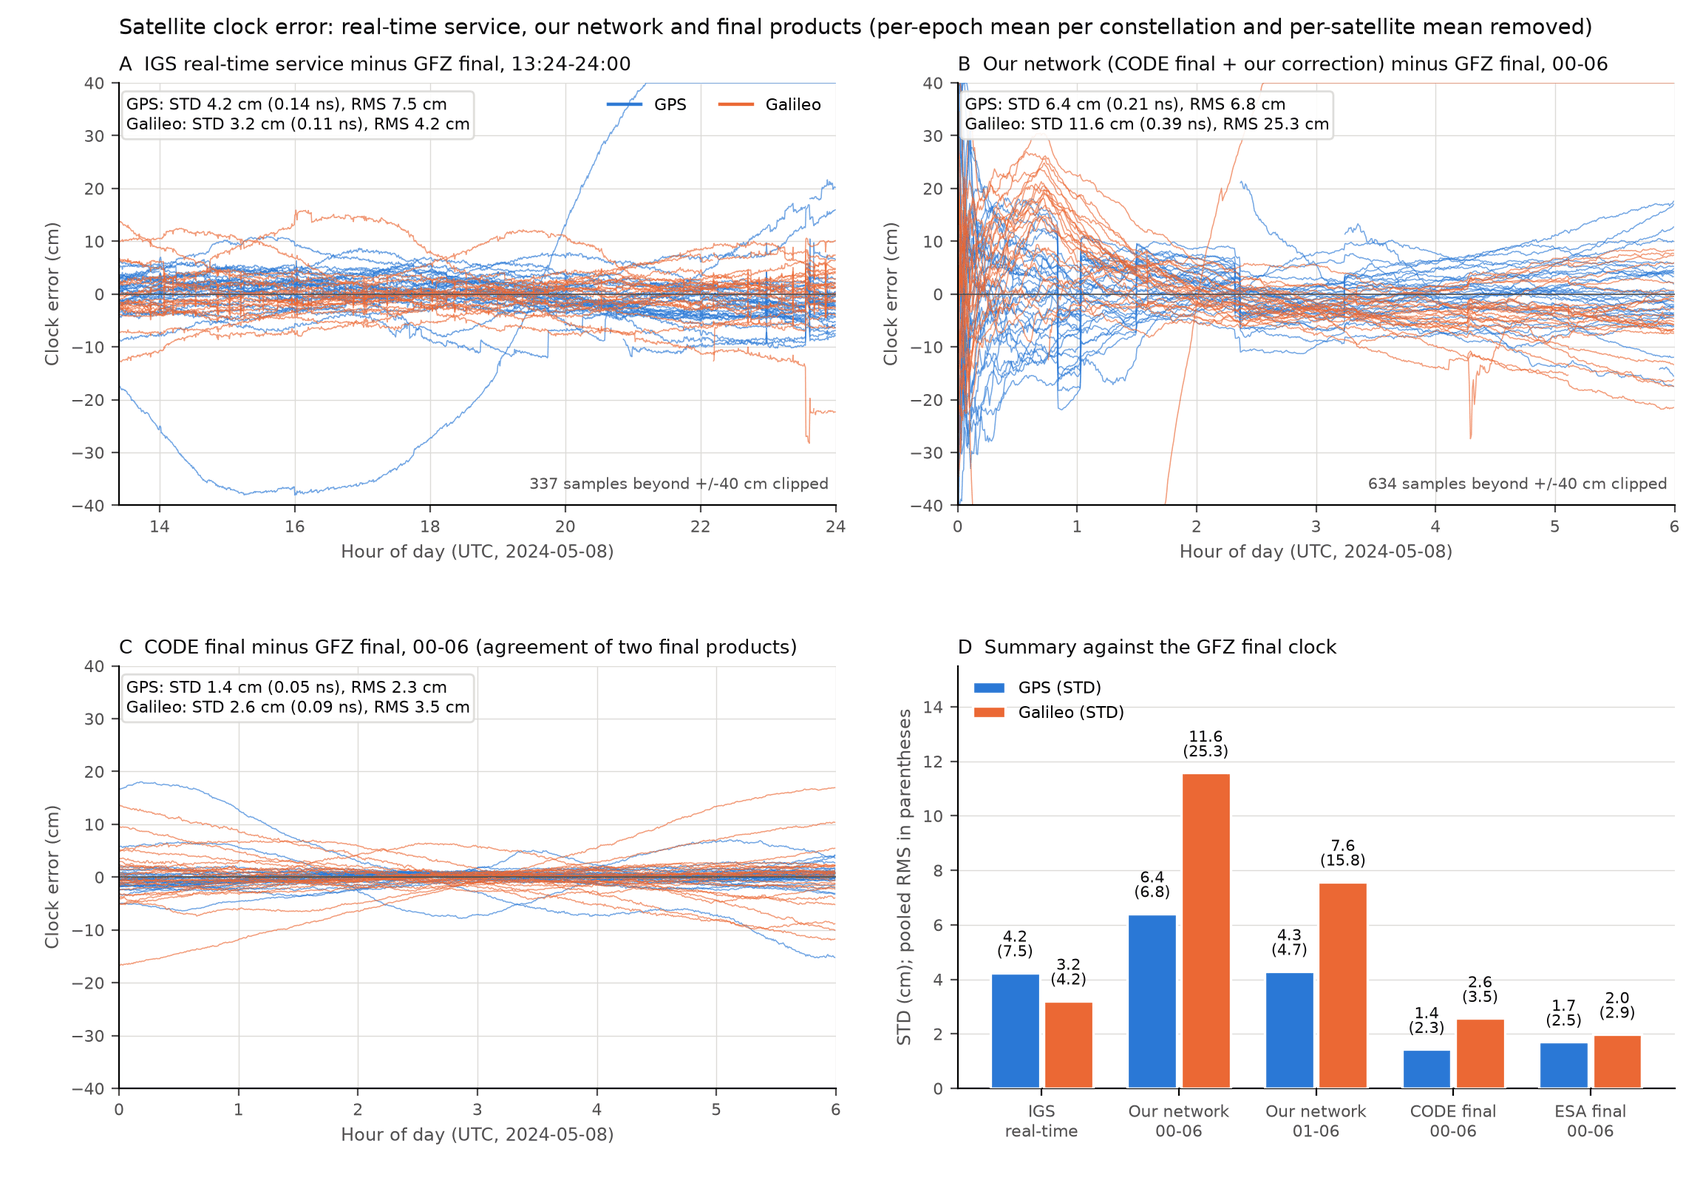
\includegraphics[width=0.62\linewidth]{clock_against_gfz.png}\hfill
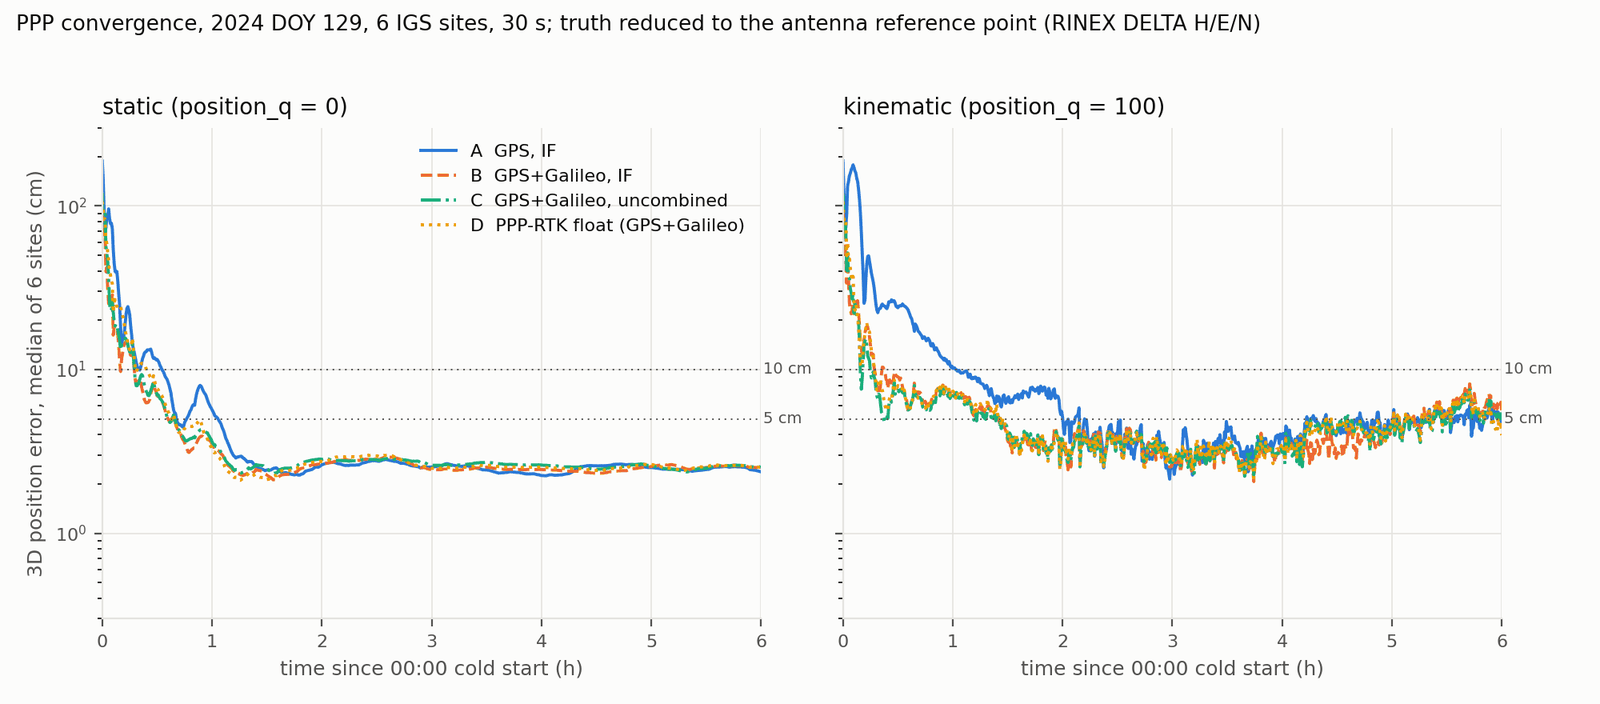
\includegraphics[width=0.36\linewidth]{ppp_convergence.png}
\caption{Left: satellite clock error against the GFZ final clock after removing the
per-system epoch mean and each satellite's mean: (A) IGS real-time service, (B) our
network, CODE final plus our correction, 00:00 to 06:00 with the first hour, (C)
CODE final, (D) summary (\texttt{results/t3/fig\_clock\_limits\_plain.png}). Right:
the PPP comparison of steps 1 to 3, median over six stations, static and moving
receiver (\texttt{results/t1/fig\_t1\_convergence.png}).}
\label{fig:l9-c}
\end{figure}

\begin{question}{census}{measure}{The test station and the 16 stations}{\ref{q:refsat}}
Run (about 2~s and 14~s):
\begin{cmd}
C:/Python313/python.exe scripts/rapid_arm.py score \
    runs/_rf0hv15_field6 runs/_rf0hv15_sim6
C:/Python313/python.exe scripts/clock_level/gcensus.py grade galpc galp galpg
\end{cmd}
Read the test station's median error by hour on both data sets, the 16 stations'
median by hour and the paired Galileo result. By what factor is hour 1 worse than
the mean of hours 2 to 6, at WTZZ00DEU and at the median station? In which mode is
WTZZ00DEU positioned (\texttt{runs/\_rf0hv15\_field6/arm.json}:
\texttt{filter.process\_noise.position\_q}, \texttt{network.closed\_loop.ar\_mode}),
and which network stations share its site?
\end{question}

\begin{question}{fivedays}{derive}{Five days from the stored grades}{\ref{q:census}}
\texttt{D:/GnssProcessorSupport/runs\_nom/mday\_galileo\_grades.txt} holds, per day
128 to 132, the 16 stations' median by hour and WTZZ00DEU by hour. From hours 2 to
6 of the five days, compute the median and the mean of the 25 sixteen-station
medians and the median of the 25 WTZZ00DEU values. On which day is WTZZ00DEU worse
than the median station in hours 4 to 6, and what does that do to ``the best
station''?
\end{question}

\begin{question}{t3}{read}{The clock against CODE and GFZ}{\ref{q:absorb} and \ref{q:hold}}
Read \texttt{results/t3/table\_clock\_report.tex} and \texttt{results/t3/results.md}
(the summary table and lines 100 to 113). Which clock is compared with which, over
which hours? Why is GFZ the reference and not CODE? Over the same hours, how does
the network's corrected clock compare with CODE's alone? What do the correlations
of the correction with (GFZ minus CODE) and (ESA minus CODE) say?
\end{question}

\begin{question}{capstone}{synthesis}{What the presentation may claim}{the whole course}
For each of five topics, state in two or three sentences what the presentation of
29~October may claim and the evidence that bounds it: (a) the model and its
per-epoch check; (b) the reference choices; (c) the satellite clock; (d) integer
ambiguities; (e) the simulated and real-data results.
\end{question}

\lessonbox{What this lesson establishes}{%
\begin{itemize}[leftmargin=*, itemsep=0pt, topsep=2pt]
\item On 8 May 2024 the test station reaches 1.0 to 1.8~cm and the median of the 16
      further stations 3.6 to 5.4~cm in hours 2 to 6, without integers.
\item Over five days the median station holds 3.8~cm; the test station is the best
      station on some days, not all, and shares its site with network stations.
\item The network's corrected clock is noisier than CODE's alone and carries no
      clock information: the user's precision is CODE's.
\end{itemize}}
